\documentclass[11pt]{article}
\usepackage[margin=1in]{geometry}
\usepackage{graphicx}
\usepackage{booktabs}
\usepackage{hyperref}
\usepackage{caption}
\usepackage{subcaption}
\title{GATE-IR Fog Synthesis: CycleGAN vs CycleDiff (75\% Blend) -- Sample Report}
\author{Preetham}
\date{\today}
\begin{document}
\maketitle

\section{Overview}
This report documents the fog-weather synthesis pipeline for the FLIR ADAS v2 thermal dataset.
Two generators are compared: a CycleGAN translator (100\% foggy) and a CycleDiff diffusion
translator (full fog plus a 75\% fog / 25\% clear blend). For each, a YOLOv8s detector was
trained in Protocol 3A (clear + synthetic foggy) and evaluated on clear vs.\ foggy test sets.

\section{Data and Synthetic Image Paths}
\begin{itemize}
  \item \textbf{Original (clear) images:} \texttt{data/flir\_adas\_v2/FLIR\_ADAS\_v2/test/clear/*.jpg} (1200 images); VTT labels in \texttt{data/flir\_adas\_v2/yolo/thermal/labels\_vtt\_test/*.txt}.
  \item \textbf{CycleGAN fog (100\%):} \texttt{data/flir\_adas\_v2/synthetic/cyclegan/fog/images/test/*.jpg} (and \texttt{train/}, \texttt{val/}); labels in \texttt{.../labels/test/*.txt}.
  \item \textbf{CycleDiff fog (full):} \texttt{data/flir\_adas\_v2/synthetic/cyclediff/fog/images/test/*.png} (train/val similarly).
  \item \textbf{CycleDiff fog (75\% blend):} \texttt{data/flir\_adas\_v2/synthetic/cyclediff\_75fog/fog/images/test/*.jpg}.
  \item \textbf{YAML configs:} \texttt{data/flir\_adas\_v2/synthetic/cyclegan/fog/synthetic\_fog.yaml}, \texttt{.../cyclediff/.../synthetic\_fog.yaml}, \texttt{.../cyclediff\_75fog/.../synthetic\_fog.yaml}.
\end{itemize}

\section{Sample Images}
Each row shows one VTT test frame: (1) original clear with ground-truth boxes, (2) CycleGAN fog,
(3) CycleDiff full fog, (4) CycleDiff 75\% blend.

\begin{figure}[htbp]
\centering
\subcaptionbox{Clear (boxed)}{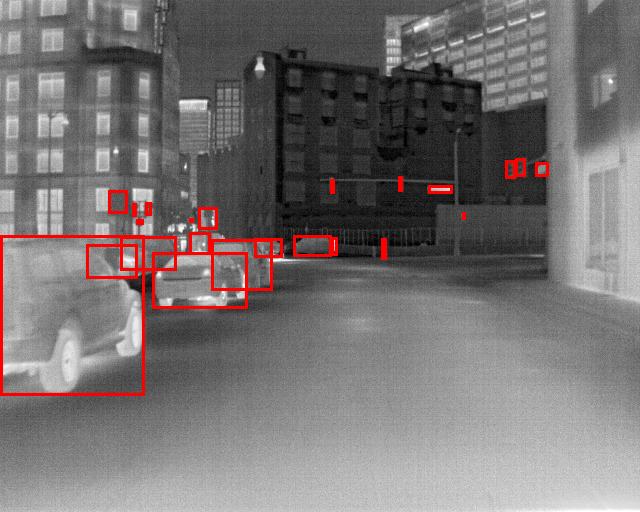
\includegraphics[width=0.24\linewidth]{report_assets/video-SCiKdG3MqZfiE292B-frame-006407-TyB7u5ZHdizi5qgyN_clear_boxed.png}}\hfill
\subcaptionbox{CycleGAN}{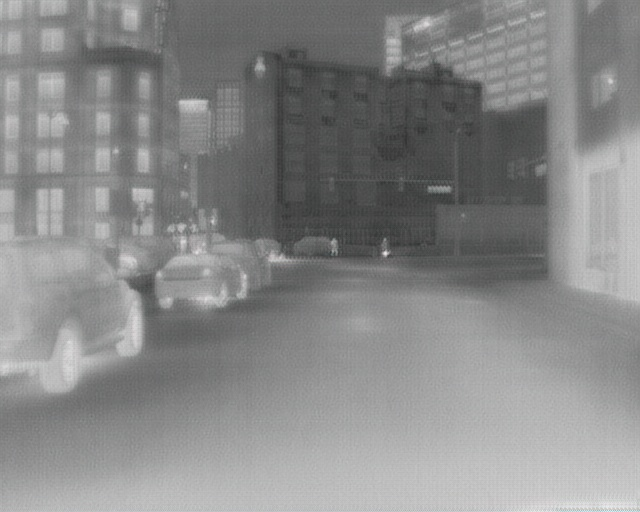
\includegraphics[width=0.24\linewidth]{report_assets/video-SCiKdG3MqZfiE292B-frame-006407-TyB7u5ZHdizi5qgyN_cyclegan.jpg}}\hfill
\subcaptionbox{CycleDiff (full)}{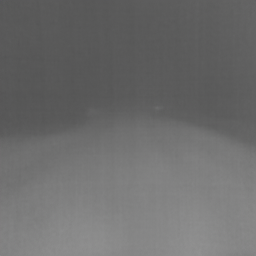
\includegraphics[width=0.24\linewidth]{report_assets/video-SCiKdG3MqZfiE292B-frame-006407-TyB7u5ZHdizi5qgyN_cyclediff.png}}\hfill
\subcaptionbox{CycleDiff (75\%)}{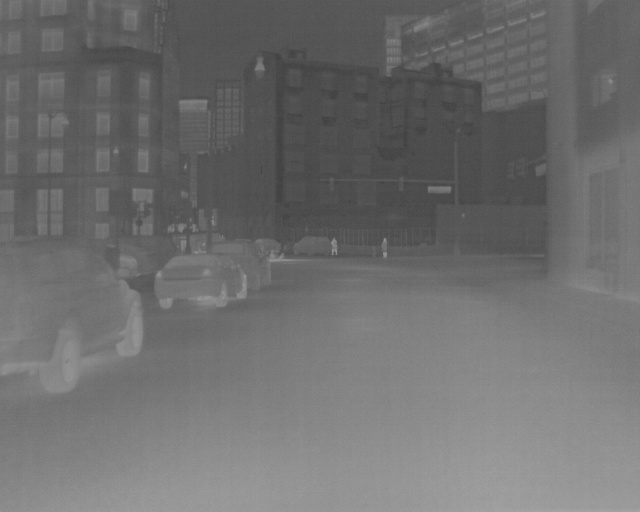
\includegraphics[width=0.24\linewidth]{report_assets/video-SCiKdG3MqZfiE292B-frame-006407-TyB7u5ZHdizi5qgyN_blend75.jpg}}
\caption{Sample frame 1.}
\end{figure}

\begin{figure}[htbp]
\centering
\subcaptionbox{Clear (boxed)}{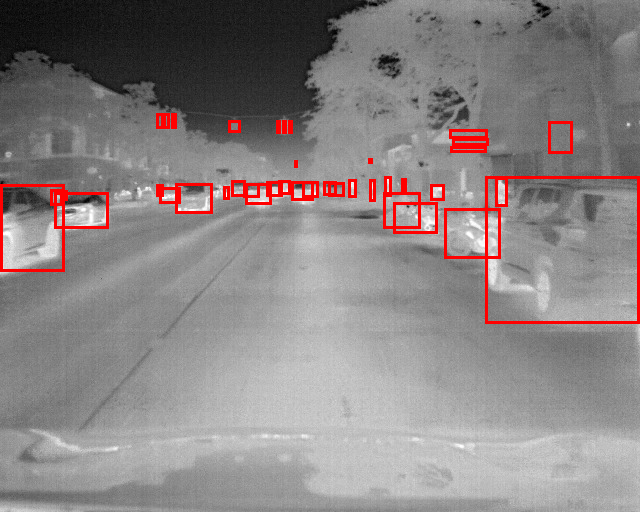
\includegraphics[width=0.24\linewidth]{report_assets/video-ZAtDSNuZZjkZFvMAo-frame-000092-ryJnHHxKPwdk3f3Wx_clear_boxed.png}}\hfill
\subcaptionbox{CycleGAN}{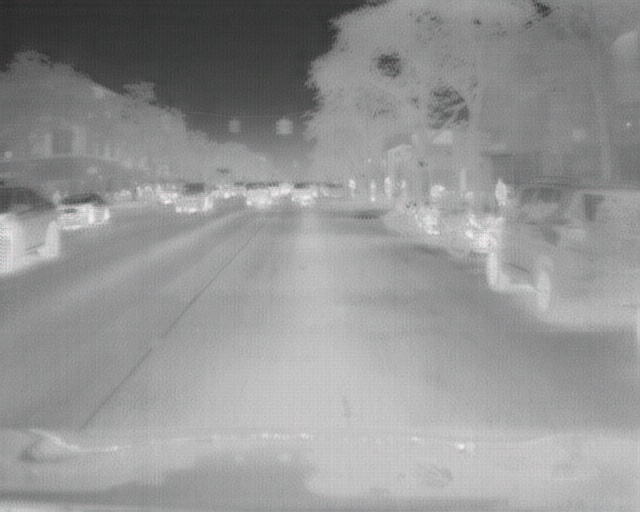
\includegraphics[width=0.24\linewidth]{report_assets/video-ZAtDSNuZZjkZFvMAo-frame-000092-ryJnHHxKPwdk3f3Wx_cyclegan.jpg}}\hfill
\subcaptionbox{CycleDiff (full)}{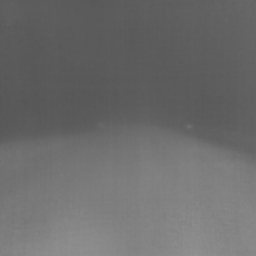
\includegraphics[width=0.24\linewidth]{report_assets/video-ZAtDSNuZZjkZFvMAo-frame-000092-ryJnHHxKPwdk3f3Wx_cyclediff.png}}\hfill
\subcaptionbox{CycleDiff (75\%)}{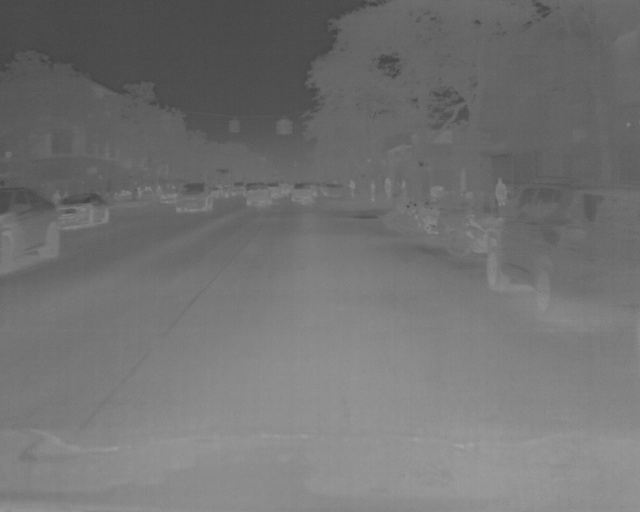
\includegraphics[width=0.24\linewidth]{report_assets/video-ZAtDSNuZZjkZFvMAo-frame-000092-ryJnHHxKPwdk3f3Wx_blend75.jpg}}
\caption{Sample frame 2.}
\end{figure}

\begin{figure}[htbp]
\centering
\subcaptionbox{Clear (boxed)}{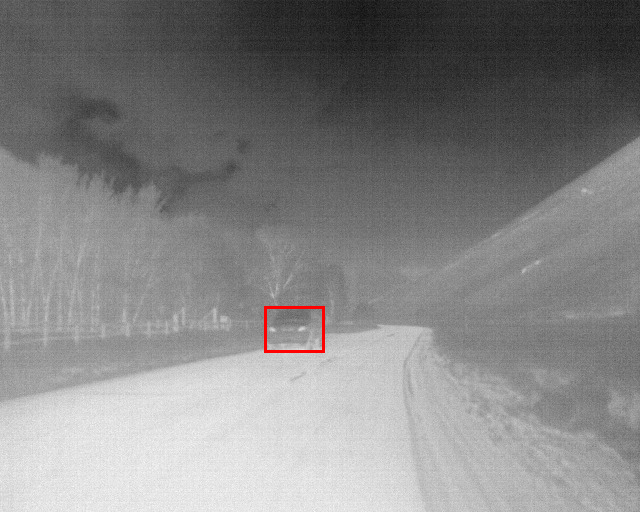
\includegraphics[width=0.24\linewidth]{report_assets/video-5RSrbWYu9eokv5bvR-frame-000351-bRrmFBB64jwa4ocDC_clear_boxed.png}}\hfill
\subcaptionbox{CycleGAN}{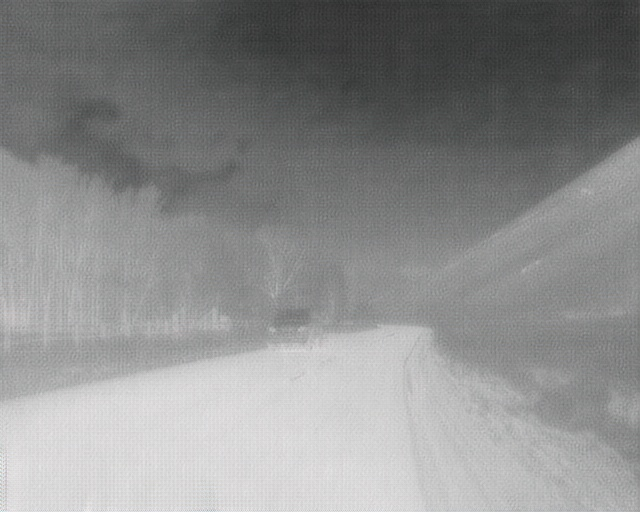
\includegraphics[width=0.24\linewidth]{report_assets/video-5RSrbWYu9eokv5bvR-frame-000351-bRrmFBB64jwa4ocDC_cyclegan.jpg}}\hfill
\subcaptionbox{CycleDiff (full)}{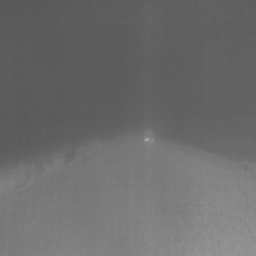
\includegraphics[width=0.24\linewidth]{report_assets/video-5RSrbWYu9eokv5bvR-frame-000351-bRrmFBB64jwa4ocDC_cyclediff.png}}\hfill
\subcaptionbox{CycleDiff (75\%)}{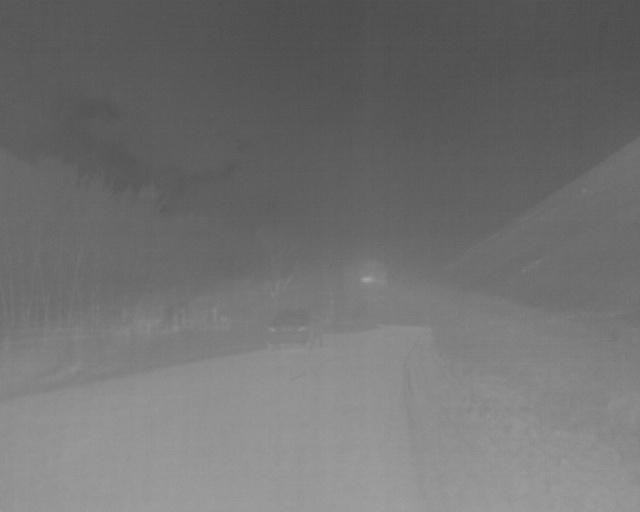
\includegraphics[width=0.24\linewidth]{report_assets/video-5RSrbWYu9eokv5bvR-frame-000351-bRrmFBB64jwa4ocDC_blend75.jpg}}
\caption{Sample frame 3.}
\end{figure}

\section{Detection Results (Protocol 3A, YOLOv8s, test set)}
\begin{table}[htbp]
\centering
\begin{tabular}{lcccc}
\toprule
Model / Test set & mAP@50-95 & mAP@50 & Precision & Recall \\
\midrule
CycleGAN fog (clear test) & 0.3274 & 0.5419 & 0.6508 & 0.5182 \\
CycleGAN fog (100\% fog test) & 0.1445 & 0.2718 & 0.4046 & 0.2819 \\
CycleDiff fog 75\% (clear test) & 0.3270 & 0.5475 & 0.6811 & 0.5271 \\
CycleDiff fog 75\% (75\% fog test) & 0.1622 & 0.3037 & 0.3952 & 0.3029 \\
CycleDiff fog (100\%, clear test) & 0.3270 & 0.5475 & 0.6811 & 0.5271 \\
CycleDiff fog (100\% fog test) & 0.0000 & 0.0000 & 0.0003 & 0.0014 \\
\bottomrule
\end{tabular}
\caption{Detection performance. CycleDiff 100\% fog model collapsed on foggy test (0.00 mAP).}
\end{table}

\section{Training Artifacts}
\begin{itemize}
  \item CycleGAN weights: \texttt{flir\_adas\_v2/runs/3a\_cyclegan\_fog-3/weights/best.pt}
  \item CycleDiff 75\% weights: \texttt{flir\_adas\_v2/runs/3a\_cyclediff\_fog-8/weights/best.pt}
  \item Result JSONs: \texttt{flir\_adas\_v2/results/3a\_cyclegan\_fog\_\{clear,adv\}.json}, \texttt{.../3a\_cyclediff\_fog\_\{clear,75\_adv,adv\}.json}.
\end{itemize}

\end{document}
